\documentclass[a4paper, 14pt]{extarticle}

% Поля
%--------------------------------------
\usepackage{geometry}
\geometry{a4paper,tmargin=2cm,bmargin=2cm,lmargin=3cm,rmargin=1cm}
%--------------------------------------


%Russian-specific packages
%--------------------------------------
\usepackage[T2A]{fontenc}
\usepackage[utf8]{inputenc} 
\usepackage[english, main=russian]{babel}
%--------------------------------------

\usepackage{textcomp}

% Красная строка
%--------------------------------------
\usepackage{indentfirst}               
%--------------------------------------             


%Graphics
%--------------------------------------
\usepackage{graphicx}
\graphicspath{ {./images/} }
\usepackage{wrapfig}
%--------------------------------------

% Полуторный интервал
%--------------------------------------
\linespread{1.3}                    
%--------------------------------------

%Выравнивание и переносы
%--------------------------------------
% Избавляемся от переполнений
\sloppy
% Запрещаем разрыв страницы после первой строки абзаца
\clubpenalty=10000
% Запрещаем разрыв страницы после последней строки абзаца
\widowpenalty=10000
%--------------------------------------

%Списки
\usepackage{enumitem}

%Подписи
\usepackage{caption} 

%Гиперссылки
\usepackage{hyperref}

\hypersetup {
	unicode=true
}

%Рисунки
%--------------------------------------
\DeclareCaptionLabelSeparator*{emdash}{~--- }
\captionsetup[figure]{labelsep=emdash,font=onehalfspacing,position=bottom}
%--------------------------------------

\usepackage{tempora}

%Листинги
%--------------------------------------
\usepackage{listings}
\lstset{
  basicstyle=\ttfamily\footnotesize, 
  %basicstyle=\footnotesize\AnkaCoder,        % the size of the fonts that are used for the code
  breakatwhitespace=false,         % sets if automatic breaks shoulbd only happen at whitespace
  breaklines=true,                 % sets automatic line breaking
  captionpos=t,                    % sets the caption-position to bottom
  inputencoding=utf8,
  frame=single,                    % adds a frame around the code
  keepspaces=true,                 % keeps spaces in text, useful for keeping indentation of code (possibly needs columns=flexible)
  keywordstyle=\bf,       % keyword style
  numbers=left,                    % where to put the line-numbers; possible values are (none, left, right)
  numbersep=5pt,                   % how far the line-numbers are from the code
  xleftmargin=25pt,
  xrightmargin=25pt,
  showspaces=false,                % show spaces everywhere adding particular underscores; it overrides 'showstringspaces'
  showstringspaces=false,          % underline spaces within strings only
  showtabs=false,                  % show tabs within strings adding particular underscores
  stepnumber=1,                    % the step between two line-numbers. If it's 1, each line will be numbered
  tabsize=2,                       % sets default tabsize to 8 spaces
  title=\lstname                   % show the filename of files included with \lstinputlisting; also try caption instead of title
}
%--------------------------------------

%%% Математические пакеты %%%
%--------------------------------------
\usepackage{amsthm,amsfonts,amsmath,amssymb,amscd}  % Математические дополнения от AMS
\usepackage{mathtools}                              % Добавляет окружение multlined
\usepackage[perpage]{footmisc}
%--------------------------------------

%--------------------------------------
%			НАЧАЛО ДОКУМЕНТА
%--------------------------------------

\begin{document}

%--------------------------------------
%			ТИТУЛЬНЫЙ ЛИСТ
%--------------------------------------
\begin{titlepage}
\thispagestyle{empty}
\newpage


%Шапка титульного листа
%--------------------------------------
\vspace*{-60pt}
\hspace{-65pt}
\begin{minipage}{0.3\textwidth}
\hspace*{-20pt}\centering

\includegraphics[width=\textwidth]{emblem}
\end{minipage}
\begin{minipage}{0.67\textwidth}\small \textbf{
\vspace*{-0.7ex}
\hspace*{-6pt}\centerline{Министерство науки и высшего образования Российской Федерации}
\vspace*{-0.7ex}
\centerline{Федеральное государственное бюджетное образовательное учреждение }
\vspace*{-0.7ex}
\centerline{высшего образования}
\vspace*{-0.7ex}
\centerline{<<Московский государственный технический университет}
\vspace*{-0.7ex}
\centerline{имени Н.Э. Баумана}
\vspace*{-0.7ex}
\centerline{(национальный исследовательский университет)>>}
\vspace*{-0.7ex}
\centerline{(МГТУ им. Н.Э. Баумана)}}
\end{minipage}
%--------------------------------------

%Полосы
%--------------------------------------
\vspace{-25pt}
\hspace{-35pt}\rule{\textwidth}{2.3pt}

\vspace*{-20.3pt}
\hspace{-35pt}\rule{\textwidth}{0.4pt}
%--------------------------------------

\vspace{1.5ex}
\hspace{-35pt} \noindent \small ФАКУЛЬТЕТ\hspace{80pt} <<Информатика и системы управления>>

\vspace*{-16pt}
\hspace{47pt}\rule{0.83\textwidth}{0.4pt}

\vspace{0.5ex}
\hspace{-35pt} \noindent \small КАФЕДРА\hspace{50pt} <<Теоретическая информатика и компьютерные технологии>>

\vspace*{-16pt}
\hspace{30pt}\rule{0.866\textwidth}{0.4pt}
  
\vspace{11em}

\begin{center}
\Large {\bf Лабораторная работа № 1} \\ 
\large {\bf по курсу <<Численные методы линейной алгебры>>} \\
\large <<Поиск минимума функции методом перебора и дихотомии>> 
\end{center}\normalsize

\vspace{8em}


\begin{flushright}
  {Студент группы ИУ9-82Б Виленский С. Д. \hspace*{15pt}\\ 
  \vspace{2ex}
  Преподаватель Посевин Д. П.\hspace*{15pt}}
\end{flushright}

\bigskip

\vfill
 

\begin{center}
\textsl{Москва 2023}
\end{center}
\end{titlepage}
%--------------------------------------
%		КОНЕЦ ТИТУЛЬНОГО ЛИСТА
%--------------------------------------

\renewcommand{\ttdefault}{pcr}

\setlength{\tabcolsep}{3pt}
\newpage
\setcounter{page}{2}

\section{Задание}\label{Sect::task}

Определить интервал, на котором функция является унимодальной, алгоритм
определения унимодальности должен принимать на вход левую и правую точку
отрезка и возвращать false — если функция на этом отрезке не унимодальная, в
противном случае true.
Реализовать поиск минимума унимодальной функции на полученном
интервале методом прямого перебора и дихотомии с заданной точностью по
вариантам. Результат должен быть представлен на графике, точки
минимизирующей последовательности должны быть выделены красным цветом.
Точность вычисления точки минимума должна варьироваться.

Найти множество точку минимума функции f(x) на отрезке.

$f(x)=x^4+3$

\section{Результаты}\label{Sect::res}

Исходный код программы представлен в листингах~\ref{lst:code1}--~\ref{lst:code2}.

\begin{figure}[!htb]
\begin{lstlisting}[language={},caption={Нахождение минимумов функции},label={lst:code1}]
using Printf
using PyPlot

function draw_plot(f, a, b, step)
    x=a:step:b
    y=f.(x)
    plot(x,y)
end

function is_unimod(f, a, b)
    eps=0.001
    xs=a:eps:b
    found_min = false
    for i in 1:length(xs)-1
        if (found_min)
            if (f(xs[i+1]) < f(xs[i]))
                return false
            end
        else
            if (f(xs[i+1]) > f(xs[i]))
                found_min = true
            end
        end
    end

\end{lstlisting}
\end{figure}

\newpage

\begin{figure}[!htb]
\begin{lstlisting}[language={},caption={Нахождение минимумов функции (продолжение)},label={lst:code2}]
    return true
end

function iter(f, a, b, eps)
    n = floor((b-a)/eps)
    step = (b-a)/n
    xs=a:step:b
    min_x = 0
    min_y = typemax(Float32)
    for x in xs
        y = f(x)
        if (y < min_y)
            min_x = x
            min_y = y
        end
    end
    @printf("(%f, %f)", min_x, min_y)
end

function dichotomy(f, a, b, eps)
    a_i = Float32(a)
    b_i = Float32(b)
    delta = eps/2
    min_x = [a_i, b_i]
    min_y = [f(a_i), f(b_i)]
    while abs(b_i - a_i) > eps
        x_1 = (a_i + b_i - delta)/2
        x_2 = (a_i + b_i + delta)/2
        if (f(x_1) <= f(x_2))
            b_i = x_2
            append!(min_x, b_i)
            append!(min_y, f(b_i))
        else
            a_i = x_1
            append!(min_x, a_i)
            append!(min_y, f(a_i))
        end
    end
    x_res = (a_i + b_i)/2 
    @printf("(%f, %f)", x_res, f(x_res))
    draw_plot(f, a, b, 0.01)
    scatter(min_x, min_y, color="r")
end

iter(f, 3, 10, 0.05)

dichotomy(f, -10, 15, 0.00000001)
\end{lstlisting}
\end{figure}

Результат запуска представлен на рисунке~\ref{fig:img1}.

\begin{figure}[!htb]
	\centering
	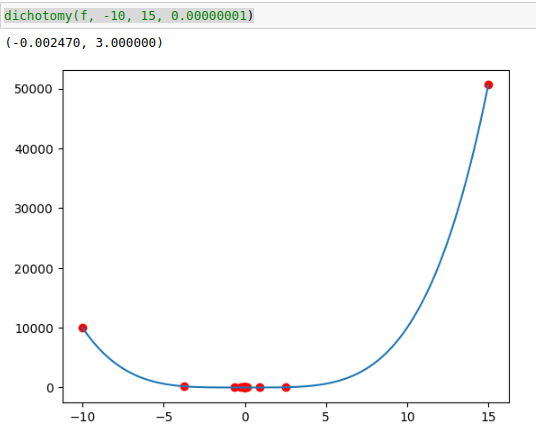
\includegraphics[width=0.8\textwidth]{img1}
\caption{Результат}
\label{fig:img1}
\end{figure}

\end{document}
